\documentclass[border=3mm,tikz,preview]{standalone}
\usepackage[utf8]{inputenc}
\usepackage{amsmath,amssymb,amsfonts}
\usepackage{graphicx}
\usepackage{tikz}
\usetikzlibrary{shapes.geometric, arrows.meta, positioning, shadows, calc, fit, backgrounds}
\usepackage{xcolor}
\begin{document}

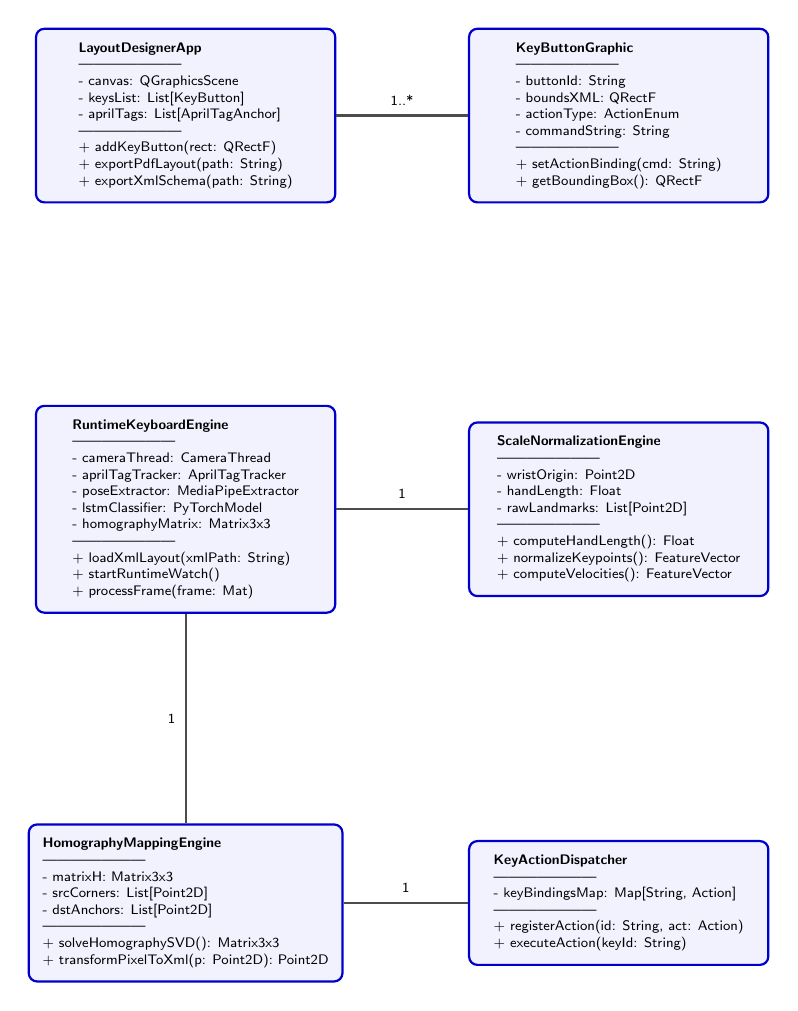
\begin{tikzpicture}[
    classbox/.style = {rectangle, draw=blue!80!black, fill=blue!5!white, thick, rounded corners=3pt, align=left, font=\sffamily\tiny, inner sep=5pt, minimum width=3.8cm},
    arrow/.style = {draw=blue!80!black, ->, >=Stealth, thick},
    assoc/.style = {draw=black!70, thick}
]

% Class: LayoutDesignerApp
\node (c_designer) [classbox] at (0, 0) {
\textbf{LayoutDesignerApp}\\
---------------------\\
- canvas: QGraphicsScene\\
- keysList: List[KeyButton]\\
- aprilTags: List[AprilTagAnchor]\\
---------------------\\
+ addKeyButton(rect: QRectF)\\
+ exportPdfLayout(path: String)\\
+ exportXmlSchema(path: String)
};

% Class: KeyButton
\node (c_key) [classbox] at (5.5, 0) {
\textbf{KeyButtonGraphic}\\
---------------------\\
- buttonId: String\\
- boundsXML: QRectF\\
- actionType: ActionEnum\\
- commandString: String\\
---------------------\\
+ setActionBinding(cmd: String)\\
+ getBoundingBox(): QRectF
};

% Class: RuntimeKeyboardEngine
\node (c_runtime) [classbox] at (0, -5) {
\textbf{RuntimeKeyboardEngine}\\
---------------------\\
- cameraThread: CameraThread\\
- aprilTagTracker: AprilTagTracker\\
- poseExtractor: MediaPipeExtractor\\
- lstmClassifier: PyTorchModel\\
- homographyMatrix: Matrix3x3\\
---------------------\\
+ loadXmlLayout(xmlPath: String)\\
+ startRuntimeWatch()\\
+ processFrame(frame: Mat)
};

% Class: ScaleNormalizationEngine
\node (c_norm) [classbox] at (5.5, -5) {
\textbf{ScaleNormalizationEngine}\\
---------------------\\
- wristOrigin: Point2D\\
- handLength: Float\\
- rawLandmarks: List[Point2D]\\
---------------------\\
+ computeHandLength(): Float\\
+ normalizeKeypoints(): FeatureVector\\
+ computeVelocities(): FeatureVector
};

% Class: HomographyMappingEngine
\node (c_homog) [classbox] at (0, -10) {
\textbf{HomographyMappingEngine}\\
---------------------\\
- matrixH: Matrix3x3\\
- srcCorners: List[Point2D]\\
- dstAnchors: List[Point2D]\\
---------------------\\
+ solveHomographySVD(): Matrix3x3\\
+ transformPixelToXml(p: Point2D): Point2D
};

% Class: ActionDispatcher
\node (c_action) [classbox] at (5.5, -10) {
\textbf{KeyActionDispatcher}\\
---------------------\\
- keyBindingsMap: Map[String, Action]\\
---------------------\\
+ registerAction(id: String, act: Action)\\
+ executeAction(keyId: String)
};

% Connections
\draw [assoc] (c_designer) -- node[above, font=\sffamily\tiny]{1..*} (c_key);
\draw [assoc] (c_runtime) -- node[above, font=\sffamily\tiny]{1} (c_norm);
\draw [assoc] (c_runtime) -- node[left, font=\sffamily\tiny]{1} (c_homog);
\draw [assoc] (c_homog) -- node[above, font=\sffamily\tiny]{1} (c_action);

\end{tikzpicture}

\end{document}
